\titleformat{\chapter}
{\normalfont\fontsize{12}{15}\centering}{Anexo\thechapter.}{0.3em}{}[]
 



\clearpage
\thispagestyle{empty}
\begin{center}
  \vspace*{\fill}
  \phantomsection
  Anexos
  \addcontentsline{toc}{chapter}{Anexos}
  \vspace*{\fill}
\end{center}
\clearpage

\appendix

\uextra{Anexo}{Dispositivo Raspberry Pi 4 Model B}
\begin{figure}[ht!]
  \centering
  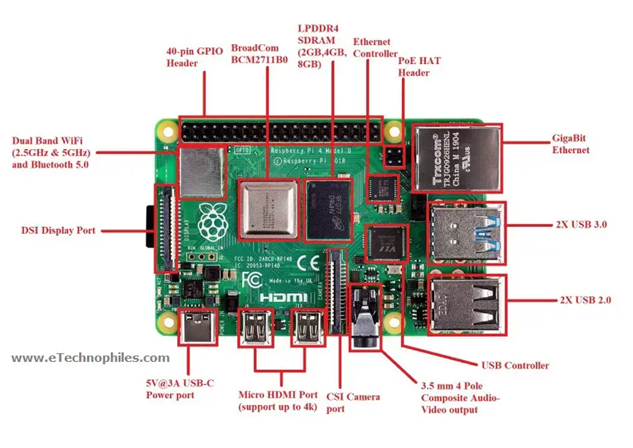
\includegraphics[width=0.95\textwidth]{Anexos/1.arquitectura-raspberry.png}
  \caption{Arquitectura del Raspberry Pi 4 Model B}
  \label{fig:raspberry-architecture}
\end{figure}

\uextra{Anexo}{Construcción del Isolation Forest (Bosque de Aislamiento)}
\begin{figure}[ht!]
  \centering
  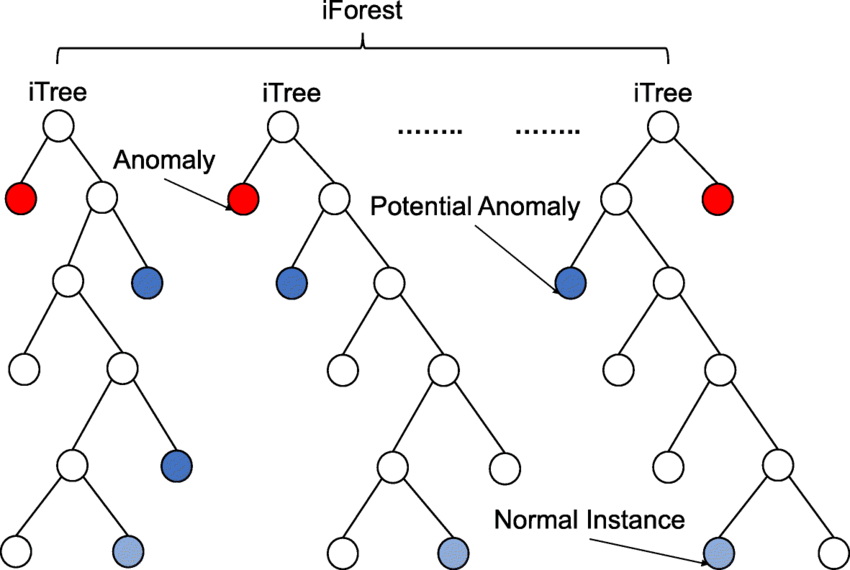
\includegraphics[width=0.95\textwidth]{Anexos/isolation-forest.png}
  \caption{Algoritmo de construcción del Isolation Forest}
  \label{fig:isolation-forest-algorithm}
\end{figure}

% \uextra{Anexo}{Categorías de sonido del modelo YAMNet}
% \uextra{Anexo}{Categorías de sonido del modelo YAMNet}
% \begin{figure}[ht!]
%   \centering
%   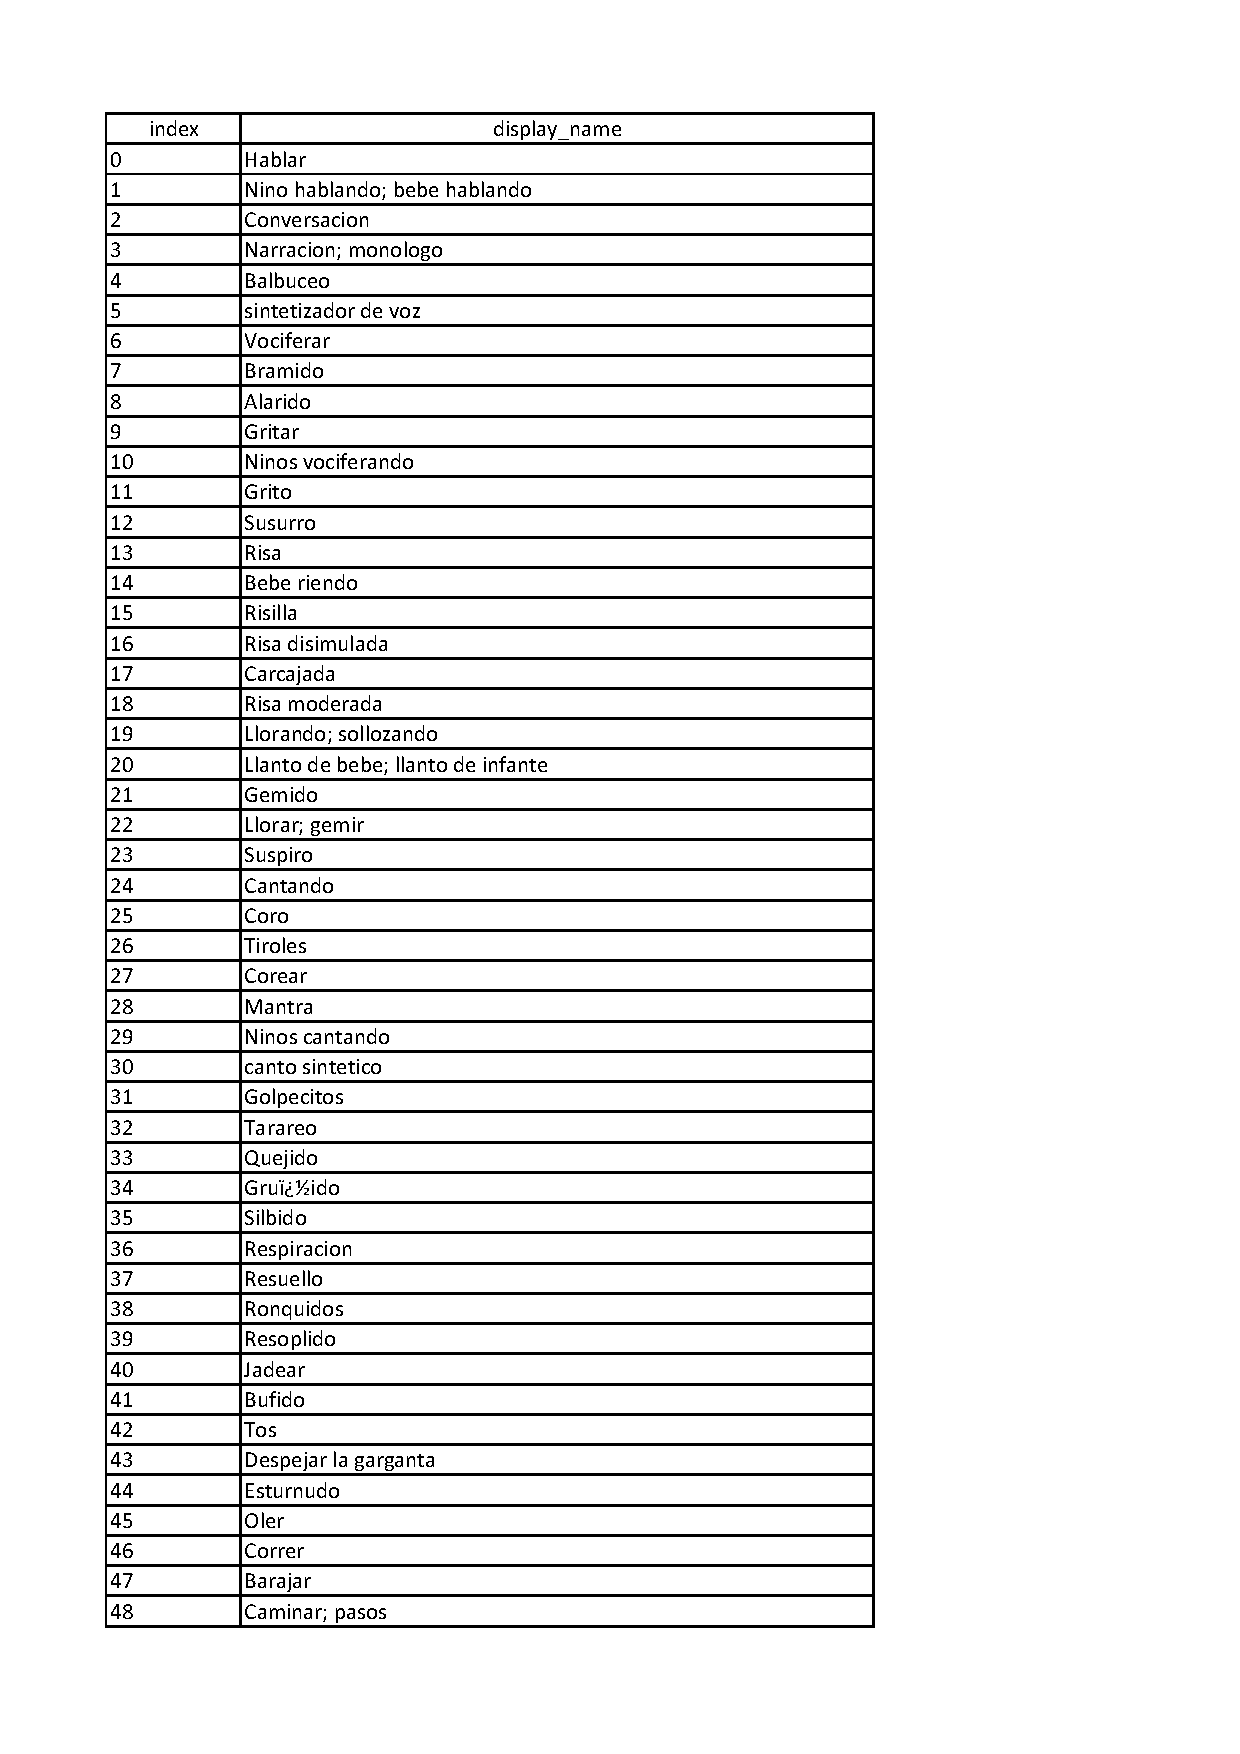
\includegraphics[width=1\textwidth]{Anexos/Clasificación de categorías.pdf}
%   \caption{Categorías de sonido del modelo YAMNet}
%   \label{fig:yamnet-categories}
% \end{figure}

\uextra{Anexo}{Numero de datos de entrenamiento por categoría de sonido}
\begin{figure}[ht!]
    \centering
    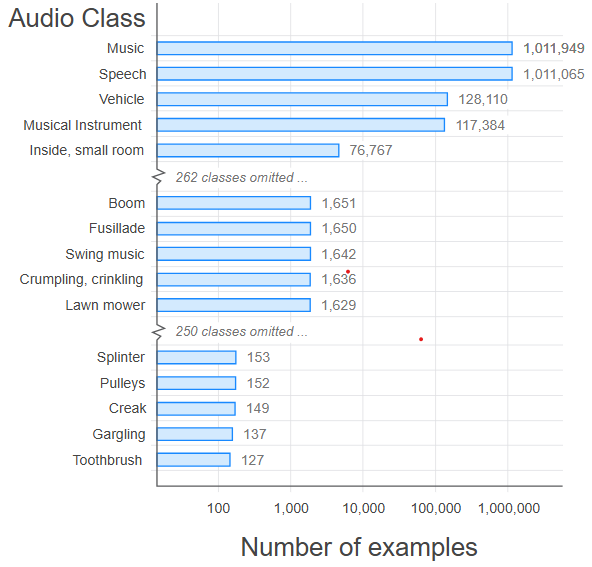
\includegraphics[width=0.95\textwidth]{Anexos/yamnet_number_examples.png}
  \caption{Número de datos de entrenamiento por categoría de sonido}
  \label{fig:training-data-per-category}
\end{figure}


\uextra{Anexo}{Categorías de sonido del modelo YAMNet}
